\section{Results}
\label{sec:results}
This chapter presents the results of the benchmarks performed.

\subsection{Read/write performance}
Due to the amount of data and the length of the tables, the results of the various read and write performance benchmarks for our files are shown in tables in Appendix \ref{readappendix} and \ref{writeappendix}. The first row of each of these tables shows the filename of the benchmarked file, while each respective column shows the time in seconds it took to read the given file. These data are used to produce the summary tables and figures below. For the read benchmark shown in figure \ref{fig:read_benchmarks}, the sub-figure of xlsx benchmark in section \textit{b} is a lot smoother compared to the rest of the sub-figures, this is due to that the benchmark time for xlsx is significantly longer compared to the other file format benchmarks. For example, each read of the xlsx file named "aggregated(v3-latest)" which is around 24.1 MB in size takes an average of 172 seconds to finish. This means that if we proceed with the planned 1,000 iterations of each benchmark, it would take 48 hours to benchmark only the largest file. Therefore, we have chosen to benchmark it only 10 times for xlsx only. In the same situation as with the Avro benchmark in sub-figure \textit{c}, the benchmark for the larger files, named aggregated\_20MB and aggregated(v3-latest), are only run 100 times instead of 1,000. Figure \ref{fig:read_benchmarks_summary} presents the summary of the results of the read benchmark using the Python Pandas library. As shown in sub-figure \textit{a}, the xlsx file format shows significantly more time to finish reading compared to the other file formats, and the trend continues as the file size increases, suppressing the other file format metrics. After excluding the xlsx format, it becomes clear that the Parquet format has the best read performance compared to the rest of the benchmarked file formats since the read time increases at a very slow rate as the file size grows bigger.

\clearpage
\begin{center}
    %\caption{CSV Pandas Read Benchmark}
    \label{table:tablereadsummary}
   \pgfplotstabletypeset[
      multicolumn names, % allows to have multicolumn names
      col sep=comma, % the seperator in our .csv file
      begin table=\begin{longtable},
      end table=\end{longtable},
      %columns={$file\_size$, csv\_mean, xlsx\_mean, avro\_mean, parquet\_mean}
      display columns/0/.style={
        column name=File Size, % name of first column
        column type={l},string type},  % use siunitx for formatting
      display columns/1/.style={
        column name=CSV Mean,
        column type={S},string type},
      display columns/2/.style={
        column name=XLSX Mean,
        column type={S},string type},
      display columns/3/.style={
        column name=Avro Mean,
        column type={S},string type},
      display columns/4/.style={
        column name=Parquet Mean,
        column type={S},string type},
      every first column/.style={column type/.add={|}{}},	% style the first column
      every head row/.style={
        before row={
        \caption{Pandas Read Benchmark}%
        \endfirsthead
        \toprule
        }, % have a rule at top
        after row={%
            \si{\string} & \si{\second}& \si{\second}& \si{\second}& \si{\second}\\ % the units seperated by &
            \midrule} % rule under units
            },
        every last row/.style={after row=\bottomrule} % rule at bottom
    ]{tables/pandas_read_result_summary.csv} % filename/path to file
\end{center}
 
\begin{figure}[H]%
    \centering
    \subfloat[\centering  CSV ]{{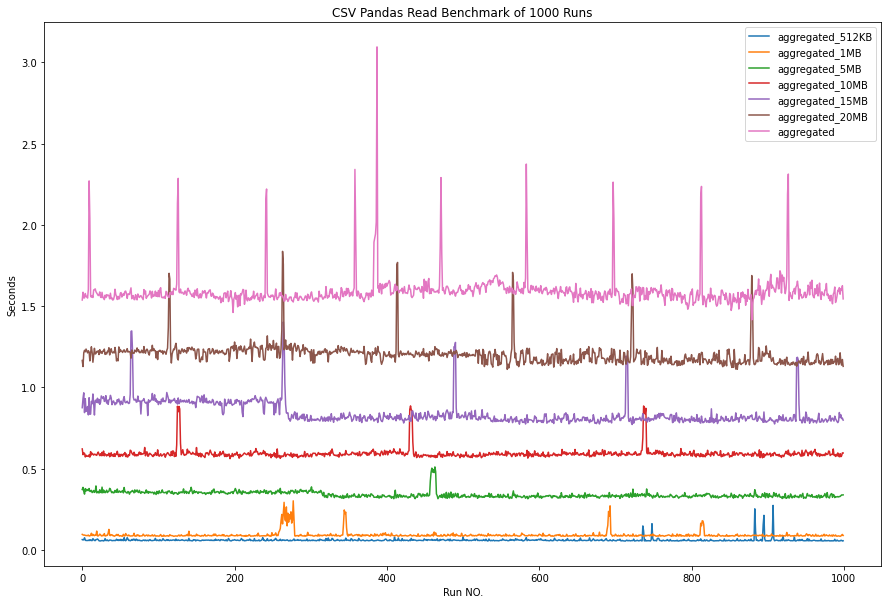
\includegraphics[width=8cm]{img/csv_read.png} }}%
    \subfloat[\centering XLSX ]{{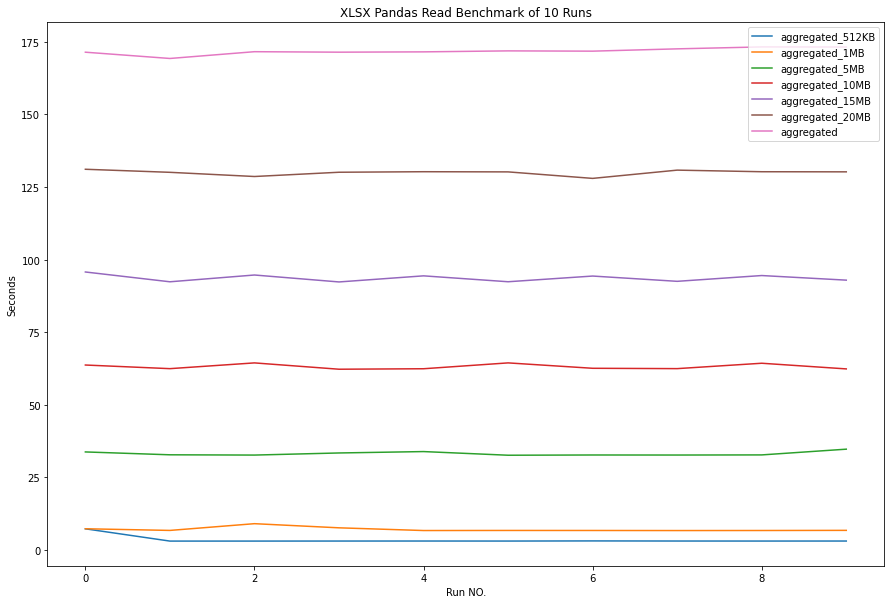
\includegraphics[width=8cm]{img/xlsx_read.png} }}%
    \quad
    \subfloat[\centering  Avro ]{{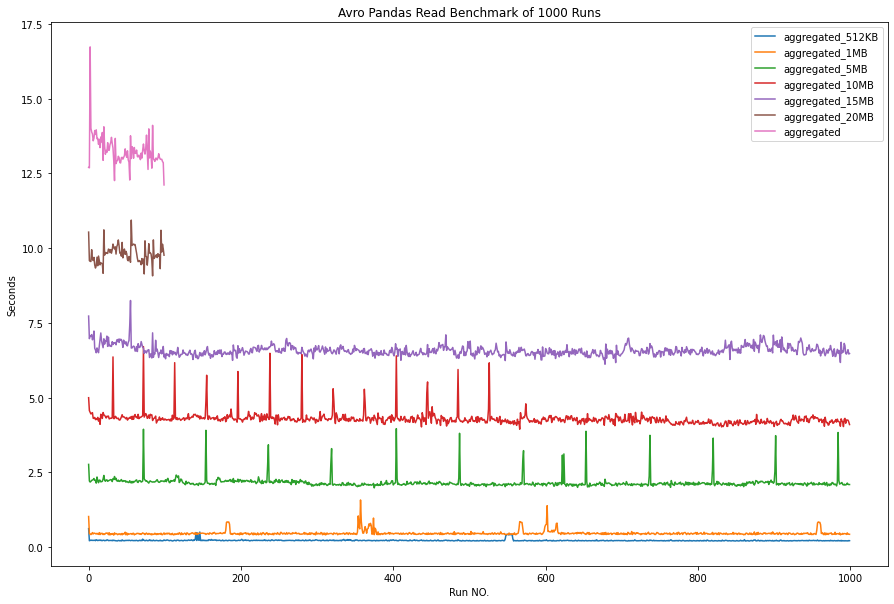
\includegraphics[width=8cm]{img/avro_read.png} }}%
    \subfloat[\centering Parquet ]{{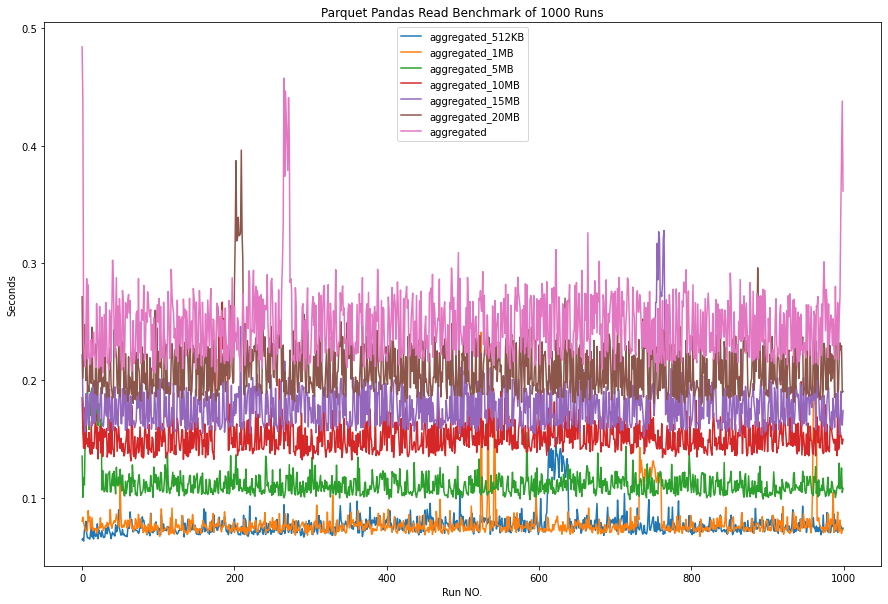
\includegraphics[width=8cm]{img/parquet_read.png} }}%
    \caption{Pandas Read Benchmark for 4 different file formats, X-axis shows each runs up to 1000th run, Y-axis shows the time it takes for each run, measured in seconds. Sub-graph b looks smooth due to the number of iterations being 10 instead of 1000, and sub-graph c has cut off for bigger file sizes because for those it was only run the benchmark 100 times instead of 1000 due to time limitation}%
    \label{fig:read_benchmarks}%
\end{figure}

\begin{figure}[H]%
    \centering
    \subfloat[\centering Read Benchmark Summary ]{{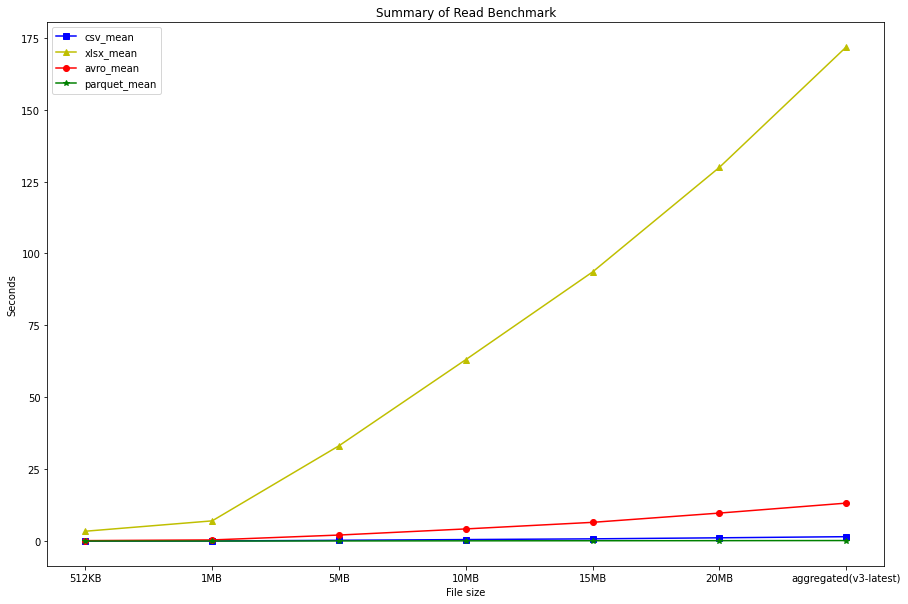
\includegraphics[width=8cm]{img/read.png} }}%
    \qquad
    \subfloat[\centering Read Benchmark Summary excluding XLSX file format]{{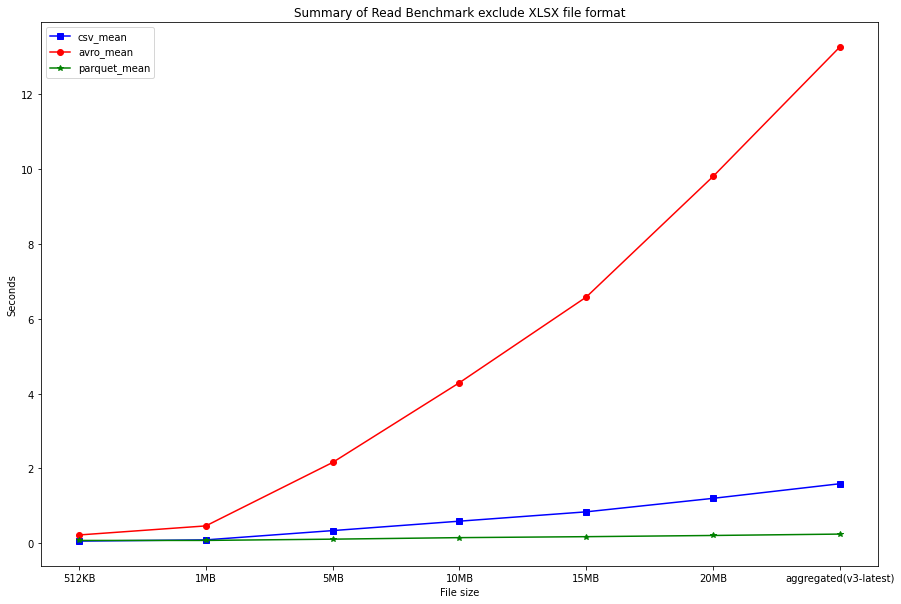
\includegraphics[width=8cm]{img/read_exlude_xlsx.png} }}%
    \caption{Summary of read benchmark using Panda for 4 different file formats, the X-axis shows the file size, starting with 0.5MB up to 24.1MB (aggregated v3-latest), while the Y-axis shows the average time it took to read the file measured in seconds}%
    \label{fig:read_benchmarks_summary}%
\end{figure}

For the write benchmark, in figure \ref{fig:write_benchmark}, the xlsx benchmark in section \textit{b} shows the same situation as its read counterpart. Meaning that we have chosen to benchmark it only 10 times for xlsx only. Due to time limitations for the Avro benchmark in sub-figure \textit{c}, the benchmarks for all sizes are only run 100 times instead of 1,000. Figure \ref{fig:write_benchmark_summary} presents a summary of the results of the write benchmark using the Python Pandas library. As shown in sub-figure \textit{a}, the xlsx file format takes significantly more time to finish writing compared to the other file formats, and the trend is only getting worse as the file size increases, suppressing the other file format's metrics. After excluding the xlsx format it becomes clear that Parquet format also has the best write performance compared to the rest of the benchmarked file formats, surprisingly the Parquet write time does not suffer as the file size increases.

\begin{center}
    %\caption{CSV Pandas Read Benchmark}
    \label{table:tablewritesummary}
   \pgfplotstabletypeset[
      multicolumn names, % allows to have multicolumn names
      col sep=comma, % the seperator in our .csv file
      begin table=\begin{longtable},
      end table=\end{longtable},
      %columns={$file\_size$, csv\_mean, xlsx\_mean, avro\_mean, parquet\_mean}
      display columns/0/.style={
        column name=File Size, % name of first column
        column type={l},string type},  % use siunitx for formatting
      display columns/1/.style={
        column name=CSV Mean,
        column type={S},string type},
      display columns/2/.style={
        column name=XLSX Mean,
        column type={S},string type},
      display columns/3/.style={
        column name=Avro Mean,
        column type={S},string type},
      display columns/4/.style={
        column name=Parquet Mean,
        column type={S},string type},
      every first column/.style={column type/.add={|}{}},	% style the first column
      every head row/.style={
        before row={
        \caption{Pandas Write Benchmark}%
        \endfirsthead
        \toprule
        }, % have a rule at top
        after row={%
            \si{\string} & \si{\second}& \si{\second}& \si{\second}& \si{\second}\\ % the units seperated by &
            \midrule} % rule under units
            },
        every last row/.style={after row=\bottomrule} % rule at bottom
    ]{tables/pandas_write_result_summary.csv} % filename/path to file
 \end{center}
 
 \begin{figure}[H]%
    \centering
    \subfloat[\centering  CSV ]{{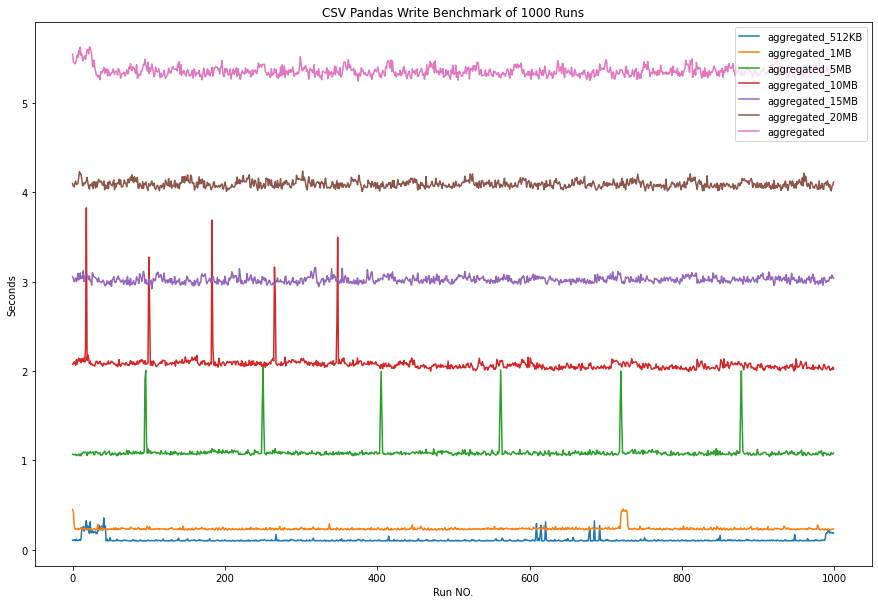
\includegraphics[width=8cm]{img/csv_write.png} }}%
    \subfloat[\centering XLSX ]{{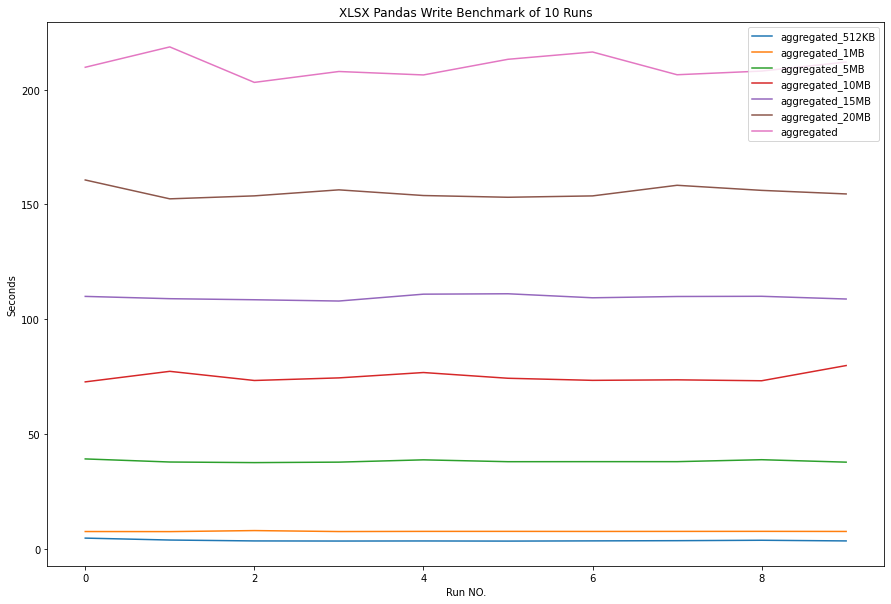
\includegraphics[width=8cm]{img/xlsx_write.png} }}%
    \quad
    \subfloat[\centering  Avro ]{{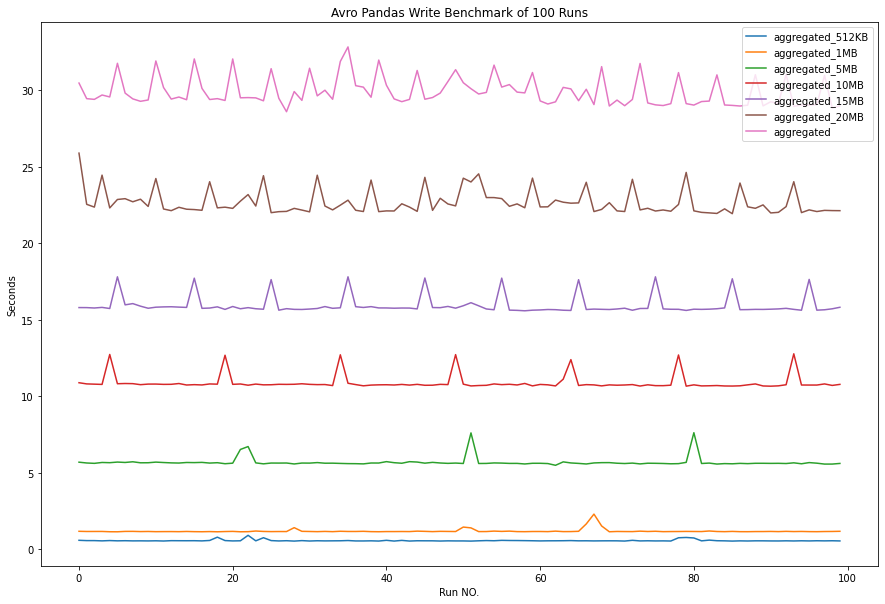
\includegraphics[width=8cm]{img/avro_write.png} }}%
    \subfloat[\centering Parquet ]{{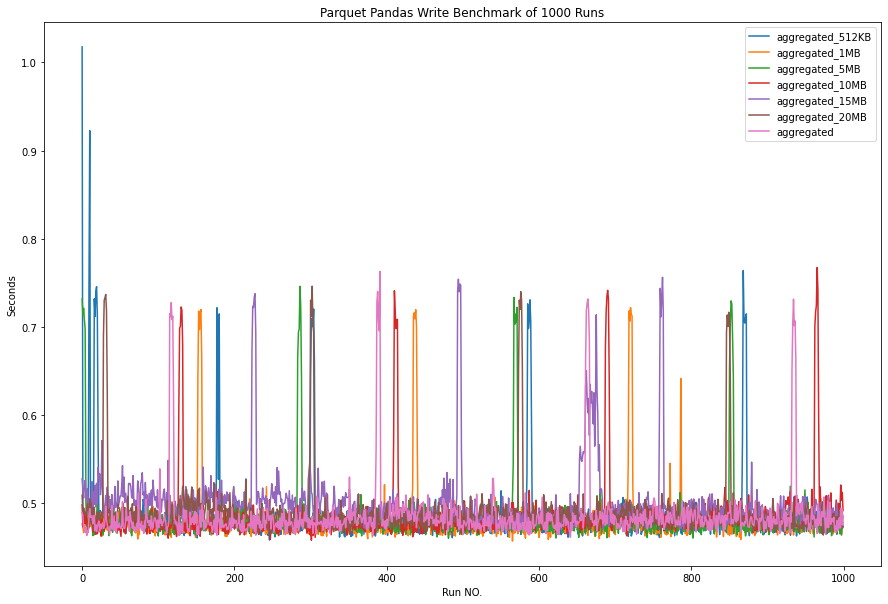
\includegraphics[width=8cm]{img/parquet_write.png} }}%
    \caption{Pandas write benchmark for 4 different file formats, the X-axis shows each run up to the 1,000th run. The Y-axis shows the time it takes for each run measured in seconds. Sub-graph \textit{b} looks smooth due to that the number of iterations is 10 instead of 1,000. Sub-graph \textit{c} also looks smoother compared to the sub-graph \textit{a} and \textit{b} because the number of iterations are  100 times instead of 1,000.}%
    \label{fig:write_benchmark}%
\end{figure}

\begin{figure}[H]%
    \centering
    \subfloat[\centering Write Benchmark Summary ]{{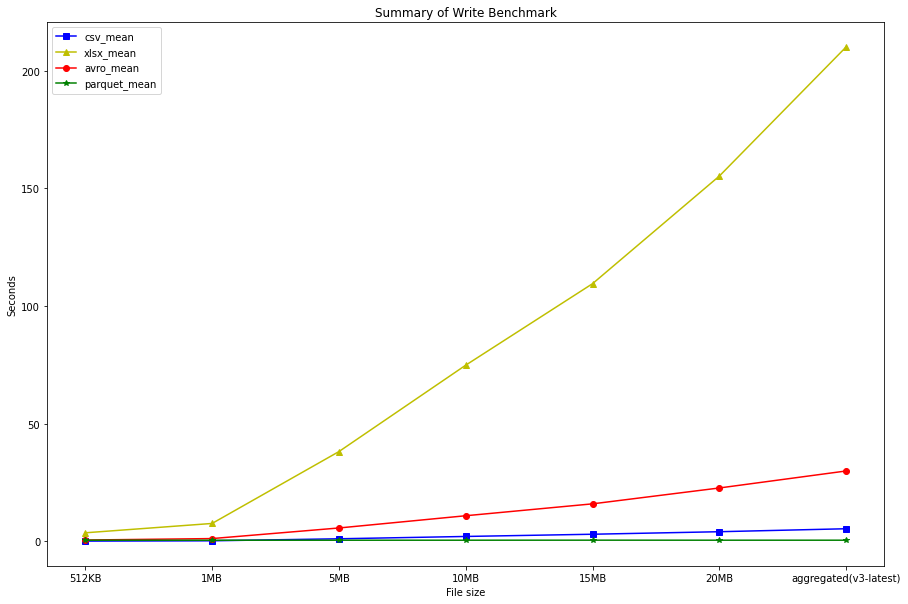
\includegraphics[width=8cm]{img/write.png} }}%
    \qquad
    \subfloat[\centering Write Benchmark Summary excluding XLSX file format]{{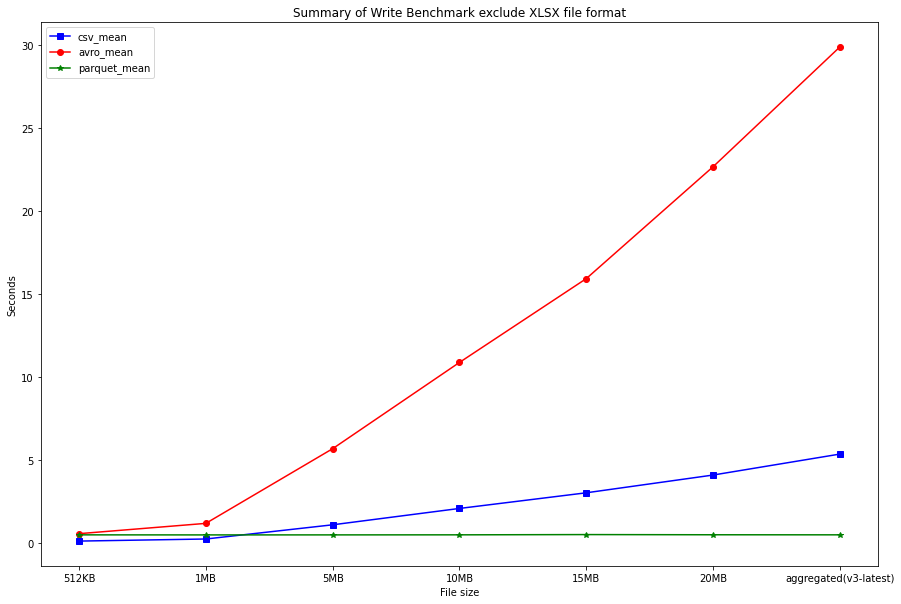
\includegraphics[width=8cm]{img/write_exlude_xlsx.png} }}%
    \caption{Summary of write benchmark using Pandas for 4 different file formats, the X-axis shows the file size starting with 0.5MB up to 24.1MB (aggregated v3-latest). The Y-axis shows the average time it took to write the file measured in seconds}%
    \label{fig:write_benchmark_summary}%
\end{figure}

\subsection{File stability}
\label{sect:file-stability-results}
 In this section, we present data from our benchmark experiment regarding the file stability explained in Section \ref{File-stability-benchmark}. Due to the significant time it takes to benchmark the xlsx format, we have excluded it from this benchmark. Table 3 shows the result of flipping a random bit in each of the files we benchmark. The first column shows the filename, while the remaining columns specify the outcome of the benchmark, ranging from \textit{Error}, \textit{No effect}, and \textit{Undetected effect}. When examining the data in Table \ref{sect:file-stability-results}, we notice that the csv files experience considerably fewer errors compared to Avro and Parquet. This is discussed in further detail in Section \ref{sec:discussion}.
\begin{center}
    \label{File-stability-benchmark}
   \pgfplotstabletypeset[
      multicolumn names, % allows to have multicolumn names
      col sep=comma, % the seperator in our .csv file
      begin table=\begin{longtable},
      end table=\end{longtable},
      %columns={$file\_size$, csv\_mean, xlsx\_mean, avro\_mean, parquet\_mean}
      display columns/0/.style={
        column name=File Name, % name of first column
        column type={l},string type},  % use siunitx for formatting
      display columns/1/.style={
        column name=File Type,
        column type={l},string type},
      display columns/2/.style={
        column name=Error,
        column type={l},string type},
      display columns/3/.style={
        column name=No effect,
        column type={l},string type},
      display columns/4/.style={
        column name=Undetected effect,
        column type={l},string type},
      every first column/.style={column type/.add={|}{}},	% style the first column
      every head row/.style={
        before row={
        \caption{Results of random bit flip when reading file}%
        \endfirsthead
        \toprule
        }, % have a rule at top
        after row={%
            \midrule} % rule under units
            },
        every last row/.style={after row=\bottomrule} % rule at bottom
    ]{tables/stability.csv} % filename/path to file
 \end{center}

\begin{figure}[h]
\centering
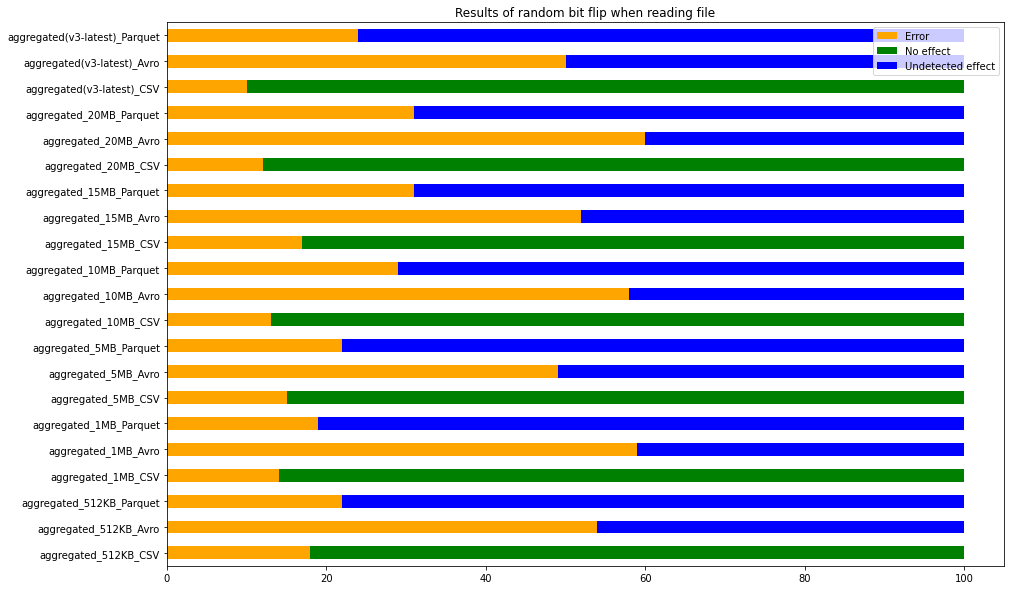
\includegraphics[scale=0.5]{img/stability.png}
\caption{Summary of file stability benchmark using Pandas for 3 different file formats including Parquet, Avro, and csv). The X-axis shows the number of runs, as well as the percentage since total of 100 runs, that were performed for each file. The Y-axis shows the file size and format, starting with 0.5MB up to 24.1MB (aggregated v3-latest)}
\label{fig:x cubed graph}
\end{figure}

\subsection{File Store Size}
The file size benchmark shown in Table 4 shows the file sizes of each file format when converted from csv format. Figure \ref{fig:size_summary} provides a visualization of the table. Since the file size difference is too large, "aggregated\_full" is therefore visualized in sub-figure \textit{b} instead of merging it with sub-figure \textit{a}. Furthermore, xlsx for "aggregated\_full" is not shown in sub-figure \textit{b} because of the lack of an effective method to convert a 20 GB csv file into xlsx format. 


\clearpage
\begin{center}
    %\caption{CSV Pandas Read Benchmark}
    \label{tablesizesummary}
   \pgfplotstabletypeset[
      multicolumn names, % allows to have multicolumn names
      col sep=comma, % the seperator in our .csv file
      begin table=\begin{longtable},
      end table=\end{longtable},
      %columns={$file\_size$, csv\_mean, xlsx\_mean, avro\_mean, parquet\_mean}
      display columns/0/.style={
        column name=File Name, % name of first column
        column type={l},string type},  % use siunitx for formatting
      display columns/1/.style={
        column name=CSV (MB),
        column type={l},string type},
      display columns/2/.style={
        column name=XLSX (MB),
        column type={l},string type},
      display columns/3/.style={
        column name=Avro (MB),
        column type={l},string type},
      display columns/4/.style={
        column name=Parquet (MB),
        column type={l},string type},
      every first column/.style={column type/.add={|}{}},	% style the first column
      every head row/.style={
        before row={
        \caption{File Store Size Benchmark}%
        \endfirsthead
        \toprule
        }, % have a rule at top
        after row={%
            \midrule} % rule under units
            },
        every last row/.style={after row=\bottomrule} % rule at bottom
    ]{tables/file_size.csv} % filename/path to file
 \end{center}
 
 \begin{figure}[H]%
    \centering
    \subfloat[\centering File Size Benchmark Summary ]{{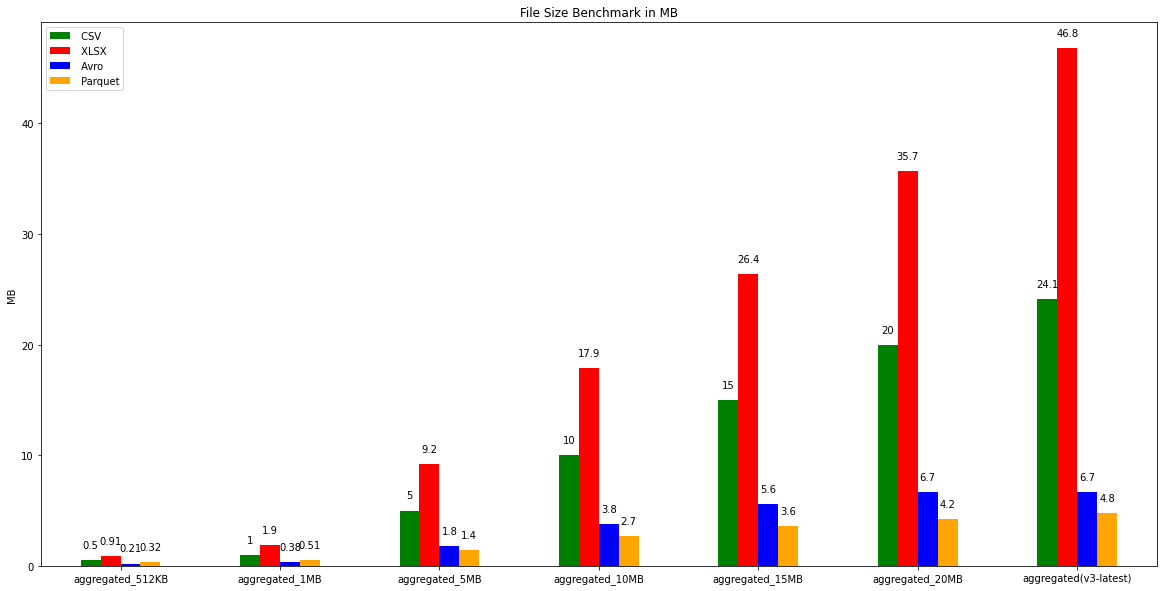
\includegraphics[width=12cm]{img/size.png} }}%
    \qquad
    \subfloat[\centering File size benchmark summary for full data format]{{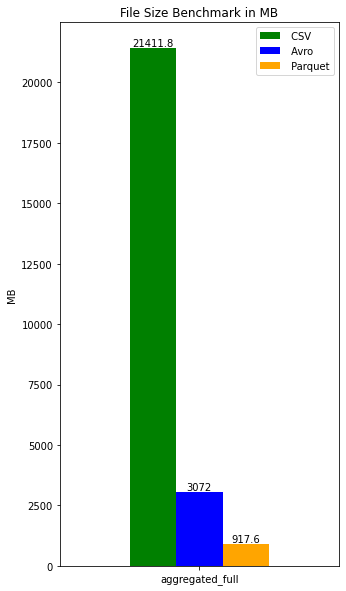
\includegraphics[width=4cm]{img/size_full.png} }}%
    \caption{File size benchmark summary of the 4 file formats in different sizes listed on the X-axis. The file size is measured in MB and shown on the Y-axis)}%
    \label{fig:size_summary}%
\end{figure}